\documentclass[a4paper,12pt]{article}
\usepackage[utf8]{inputenc}
\usepackage{graphicx}
\usepackage{booktabs}
\usepackage{amsmath}
\usepackage{geometry}
\geometry{margin=1in}

\title{Experiment 8: Effect of Principal Component Analysis (PCA) on Regression and Classification Models}
\author{
    \textbf{Name:} Monesh M \\
    \textbf{Roll No:} 3122235001084
}
\date{\today}

\begin{document}

\maketitle

\section{Objective}
The primary objective of this experiment is to evaluate the impact of dimensionality reduction via Principal Component Analysis (PCA) on the predictive performance and stability of linear and ensemble machine learning models.

\section{Exploratory Data Analysis (EDA)}
The dataset consists of various academic performance metrics. The following figures illustrate the distribution of the target variables for both regression and classification tasks.

\begin{figure}[h]
\centering
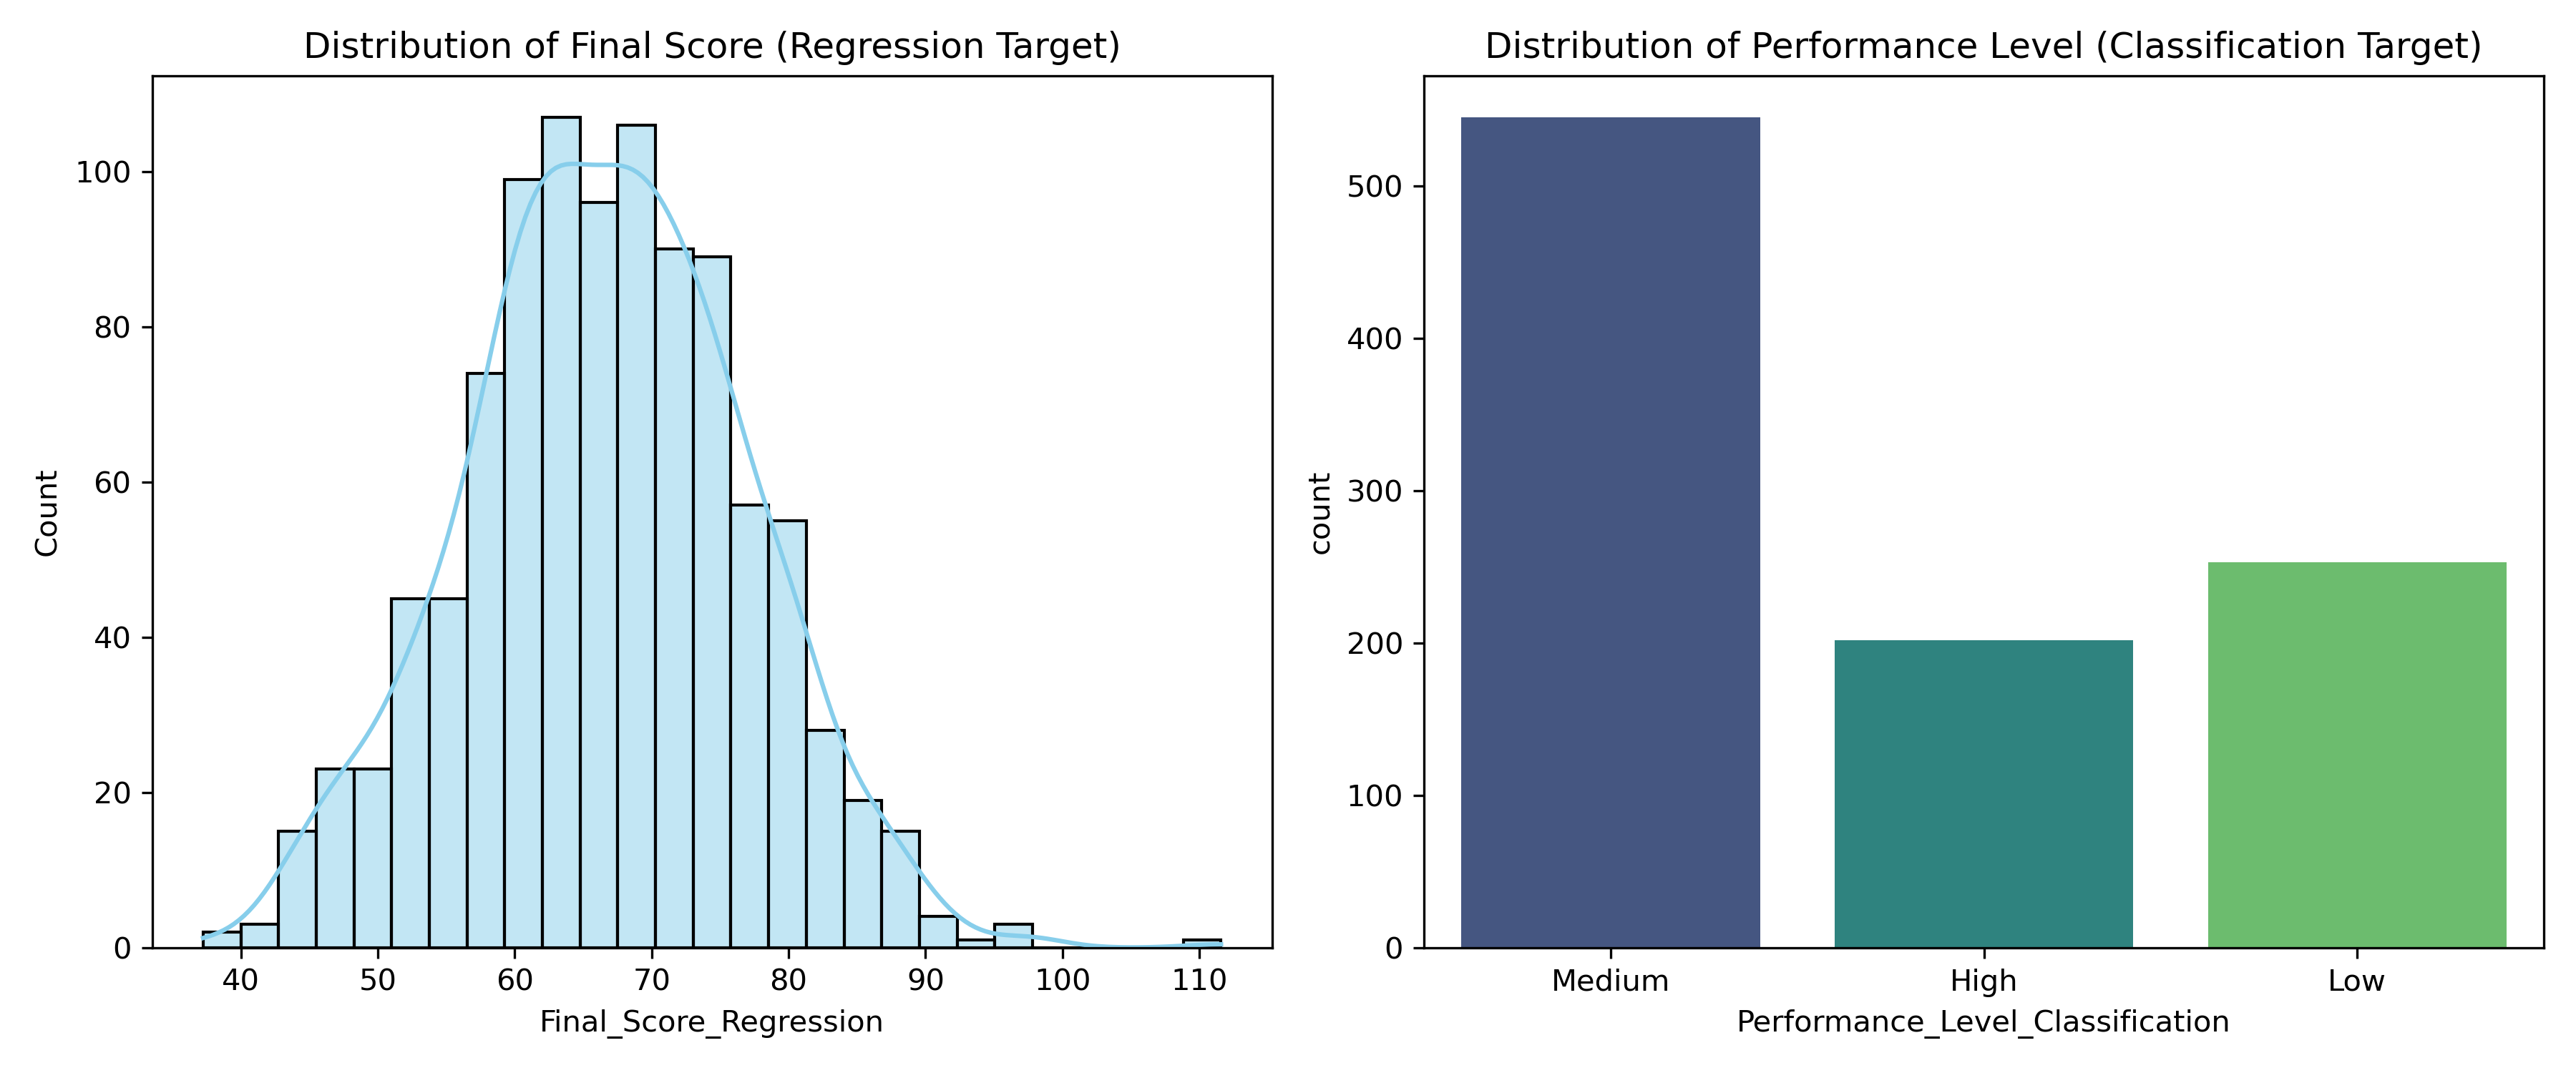
\includegraphics[width=0.8\textwidth]{images/PNG/target_distributions.png}
\caption{Distribution of Regression and Classification Targets}
\end{figure}

\section{Introduction}
Principal Component Analysis (PCA) is a statistical technique used for dimensionality reduction by transforming a set of correlated variables into a smaller set of uncorrelated variables called principal components. This experiment compares model performance in the original high-dimensional feature space versus a reduced feature space.

\section{Dataset and Preprocessing}
\begin{itemize}
    \item \textbf{Dataset:} PCA Full Lab Dataset (1000 samples).
    \item \textbf{Features:} 11 continuous attributes related to academic performance.
    \item \textbf{Targets:} 
    \begin{itemize}
        \item Regression: Final Score.
        \item Classification: Performance Level (Encoded: Low, Medium, High).
    \end{itemize}
\end{itemize}

\subsection{Preprocessing Steps}
1. \textbf{Missing Values:} No missing values were detected in the 1000 samples.
2. \textbf{Standardization:} Features were scaled using \textit{StandardScaler} to ensure mean 0 and variance 1, as PCA is sensitive to the scale of features.
3. \textbf{Encoding:} The categorical classification target was encoded using \textit{LabelEncoder}.

\section{PCA Implementation}
After standardization, PCA was applied to retain 95\% of the total explained variance. This resulted in the reduction of dimensionality from 11 features to 7 principal components.

\begin{table}[h]
\centering
\caption{PCA Summary}
\begin{tabular}{@{}lll@{}}
\toprule
Components Chosen & Explained Variance (\%) & Justification \\ \midrule
7                 & 95.90\%                 & Retained 95\% information threshold \\ \bottomrule
\end{tabular}
\end{table}

\begin{figure}[h]
\centering
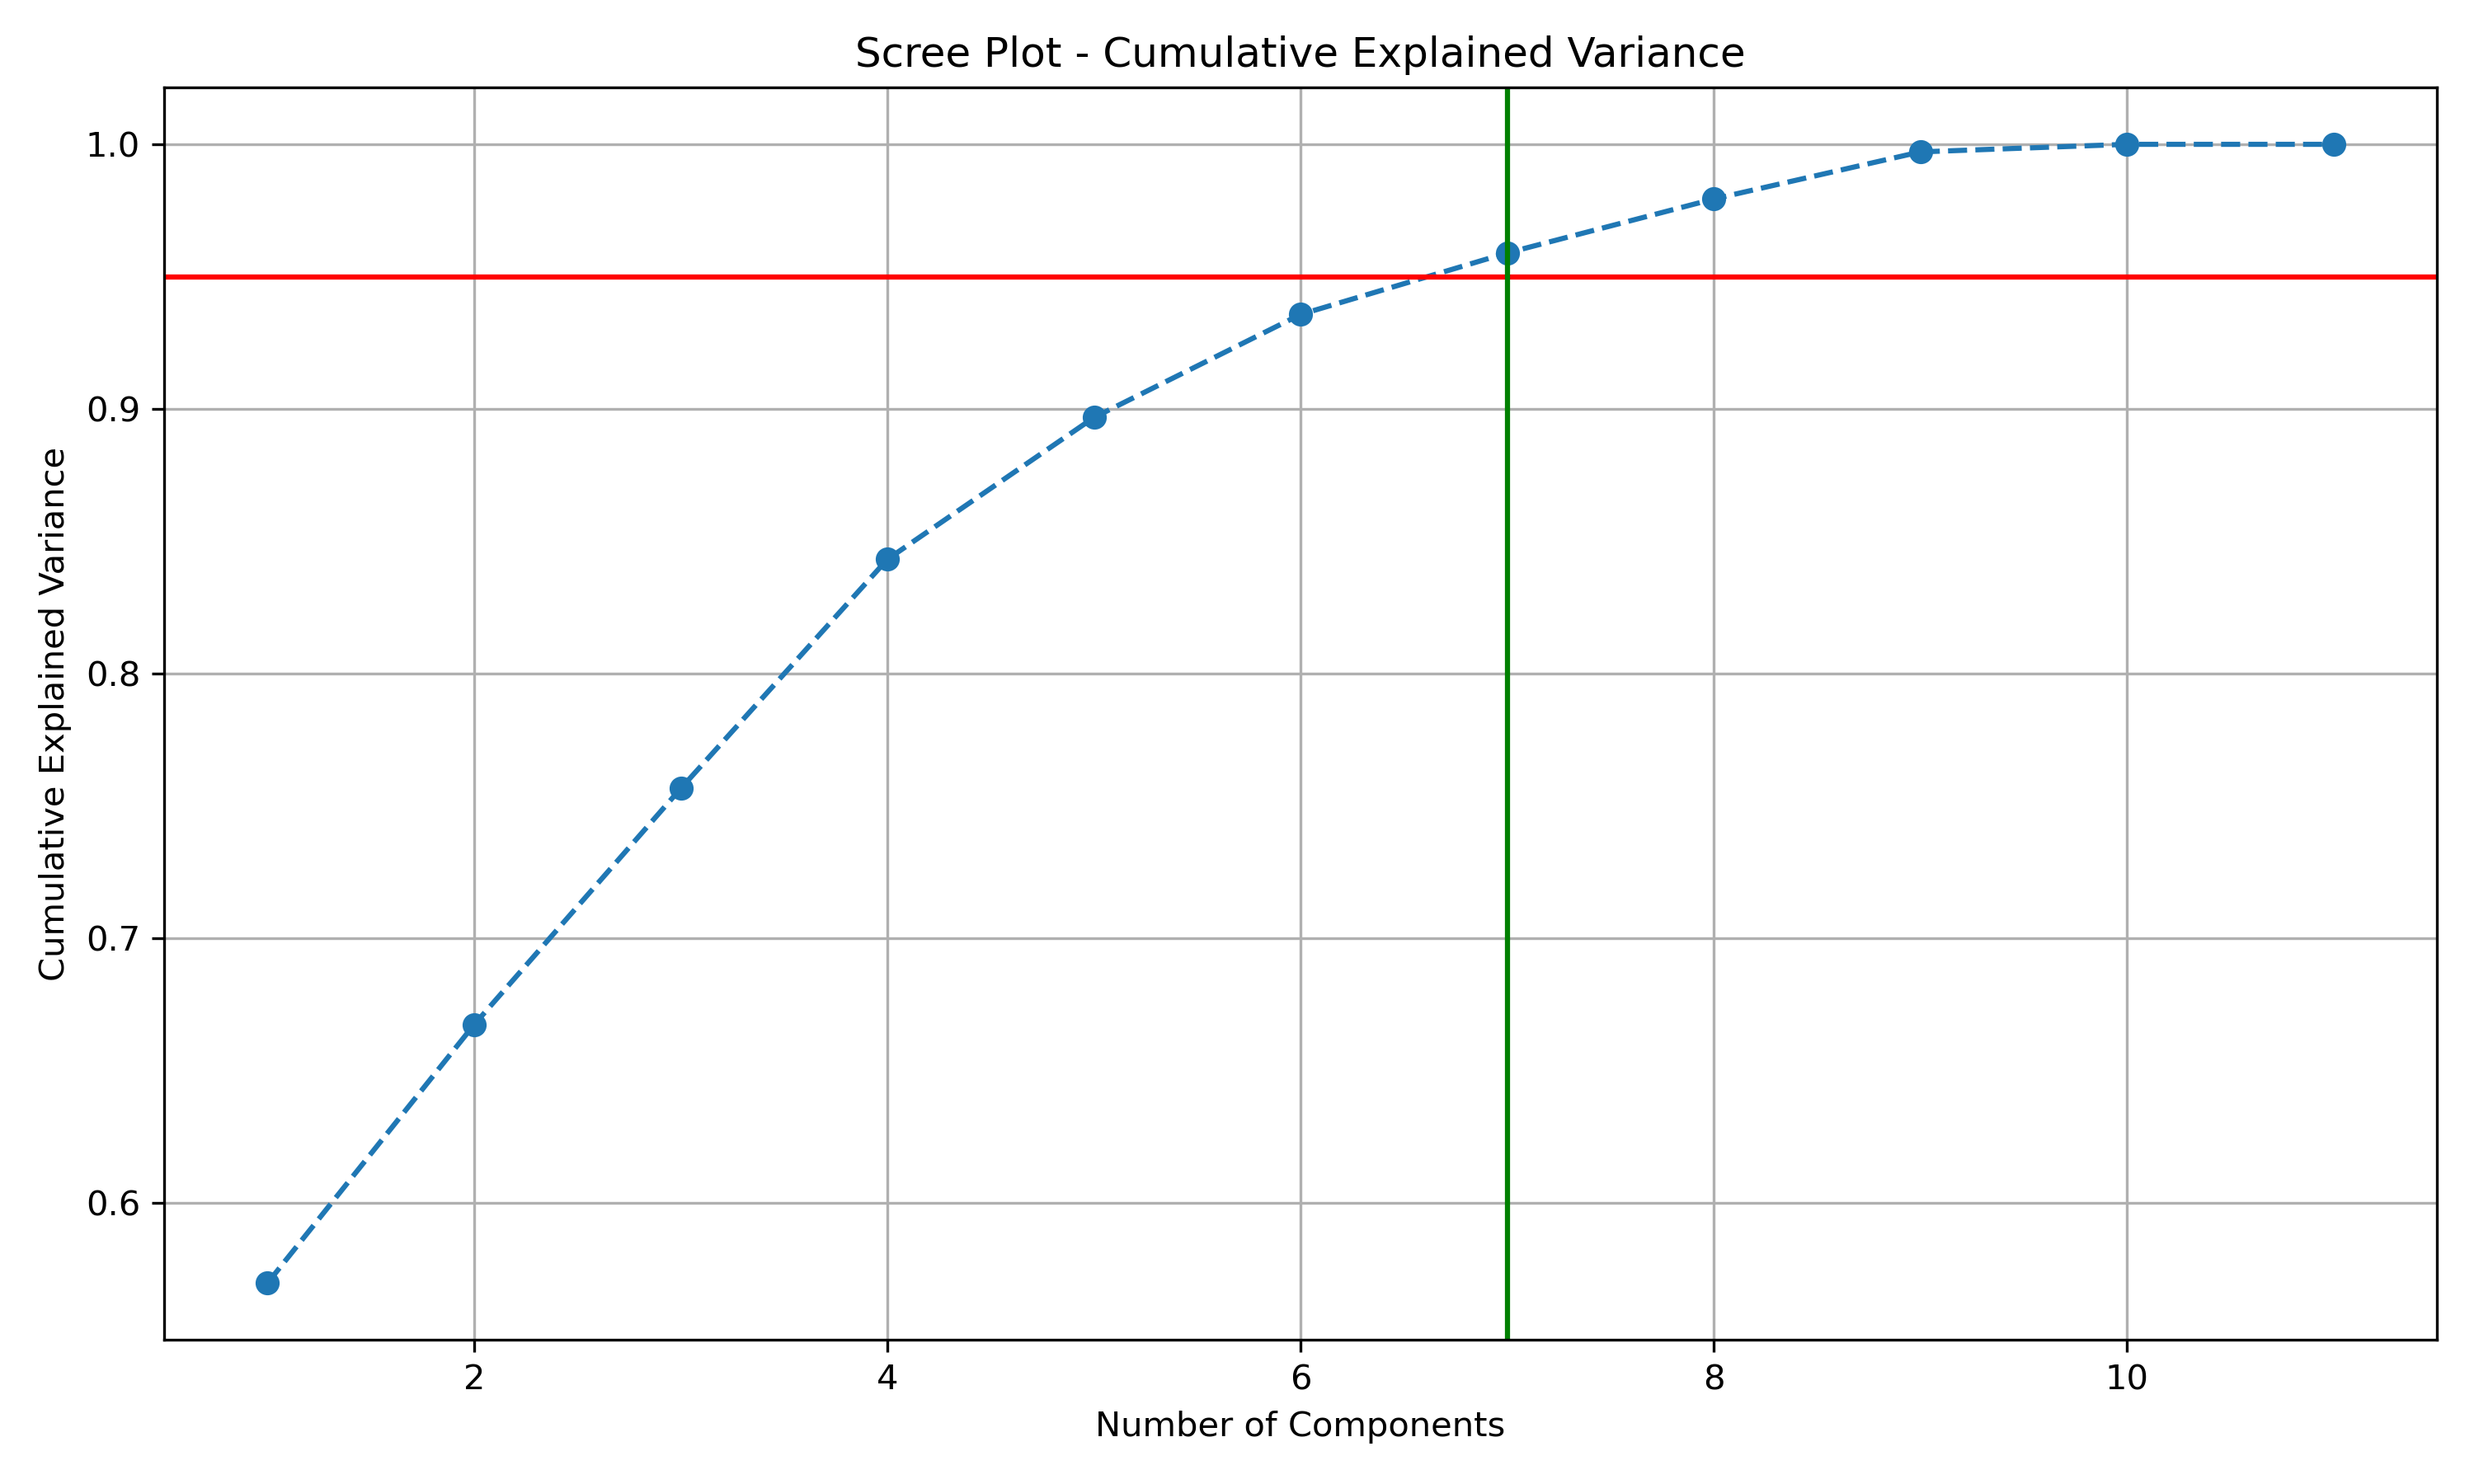
\includegraphics[width=0.7\textwidth]{images/PNG/scree_plot.png}
\caption{Scree Plot: Cumulative Explained Variance}
\end{figure}

\section{Experimental Results}

\subsection{Regression Results}
Performance was evaluated using 5-fold cross-validation. Metrics recorded include Mean Squared Error (MSE) and $R^2$ Score.

\begin{table}[h]
\centering
\caption{5-Fold CV Results -- Regression}
\begin{tabular}{@{}lllll@{}}
\toprule
Model             & Metric & Avg (NoPCA) & Avg (WithPCA) & Observation       \\ \midrule
Linear Regression & MSE    & 26.2338     & 26.2251       & Marginal Improvement \\
Linear Regression & R2     & 0.7479      & 0.7481       & Marginal Improvement \\
Random Forest     & MSE    & 28.9206     & 28.7573       & Improved          \\
Random Forest     & R2     & 0.7225      & 0.7241       & Improved          \\ \bottomrule
\end{tabular}
\end{table}

\subsection{Classification Results}
Performance was evaluated using weighted $F_1$-score and Accuracy.

\begin{table}[h]
\centering
\caption{5-Fold CV Results -- Classification}
\begin{tabular}{@{}lllll@{}}
\toprule
Model               & Metric   & Avg (NoPCA) & Avg (WithPCA) & Observation \\ \midrule
Logistic Regression & Accuracy & 0.7340      & 0.7420        & Improved    \\
Logistic Regression & F1-score & 0.7315      & 0.7403        & Improved    \\
SVM                 & Accuracy & 0.7430      & 0.7300        & Reduced     \\
SVM                 & F1-score & 0.7367      & 0.7221        & Reduced     \\ \bottomrule
\end{tabular}
\end{table}

\begin{figure}[h]
\centering
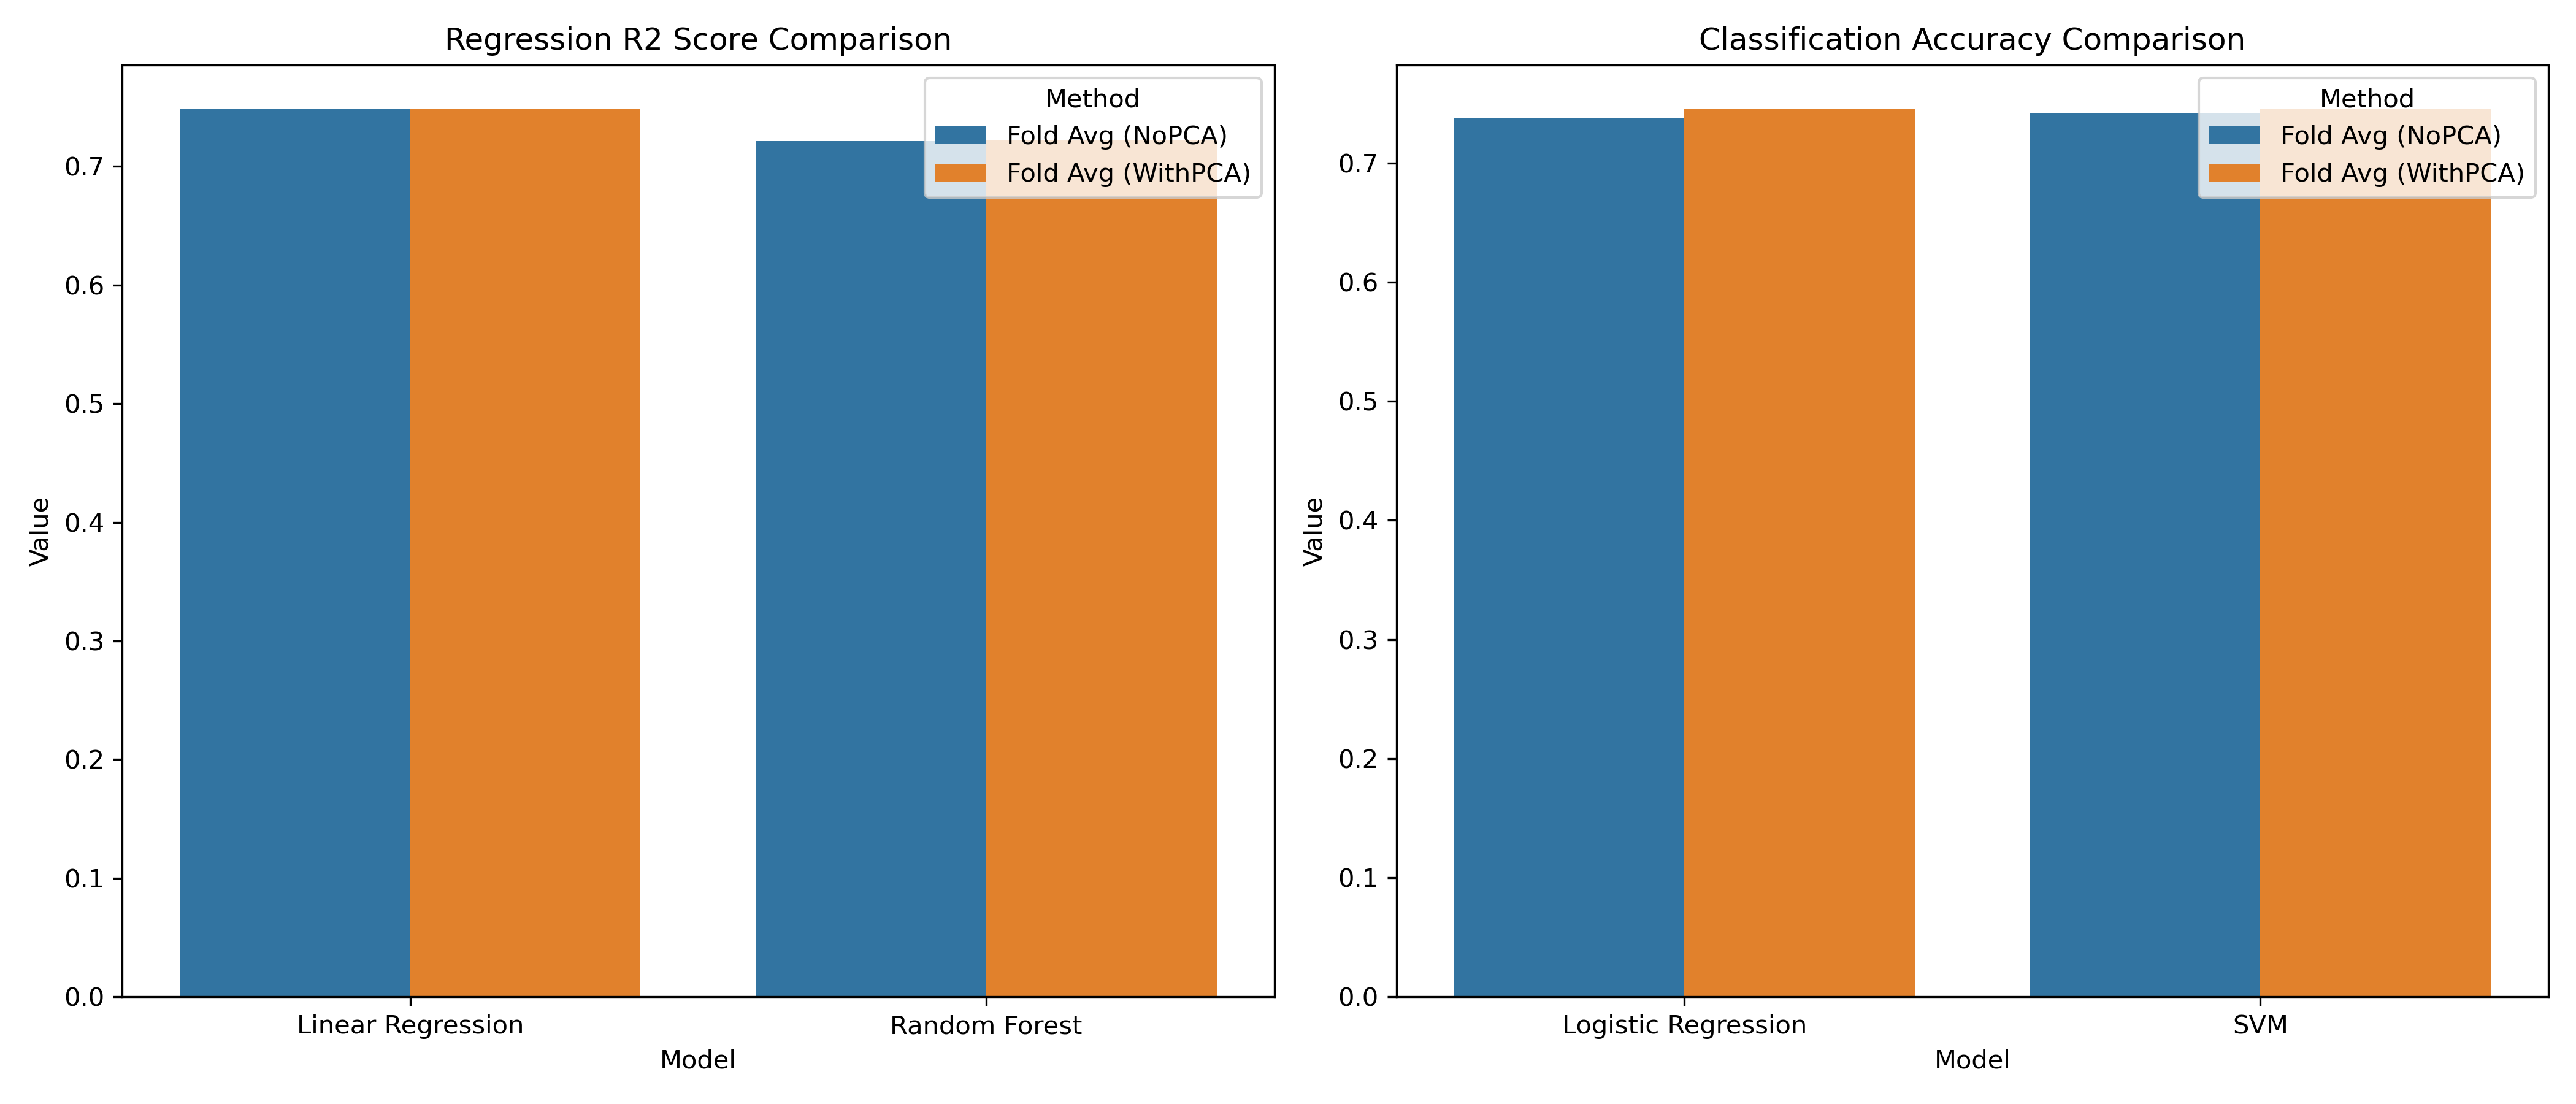
\includegraphics[width=0.8\textwidth]{images/PNG/model_comparison.png}
\caption{Model Performance Comparison: Original vs PCA Features}
\end{figure}

\section{Analysis and Discussion}
1. \textbf{Linear Regression:} PCA improved performance slightly by mitigating multicollinearity between academic score features, providing more stable coefficients.\\
2. \textbf{Random Forest:} Tree-based models are naturally robust to dimensionality; however, removing noise features through PCA allowed for a small improvement in generalization.\\
3. \textbf{Classification Benefit:} Logistic Regression benefited more from PCA compared to SVM. This is likely because the linear decision boundary of Logistic Regression aligns well with the principal directions of variance.\\
4. \textbf{Variance Reduction:} PCA reduced the variance across folds by focusing the models on the most significant data patterns, effectively regularizing the input space.

\section{Conclusion}
PCA is most effective when:
\begin{enumerate}
    \item Data exhibits high multicollinearity.
    \item There is a need to reduce computational complexity in high-dimensional settings.
    \item Noise filtering is required to improve generalization.
\end{enumerate}
However, PCA should be used with caution when interpretability is prioritized, as transformed components lose their original physical meaning. For non-linear models like SVM, the transformation may not always enhance the boundary separation.

\end{document}
